% Created 2019-01-27 dom 15:06
% Intended LaTeX compiler: pdflatex
\documentclass[xcolor={usenames,svgnames,dvipsnames}]{beamer}
\usepackage[utf8]{inputenc}
\usepackage[T1]{fontenc}
\usepackage{graphicx}
\usepackage{grffile}
\usepackage{longtable}
\usepackage{wrapfig}
\usepackage{rotating}
\usepackage[normalem]{ulem}
\usepackage{amsmath}
\usepackage{textcomp}
\usepackage{amssymb}
\usepackage{capt-of}
\usepackage{hyperref}
\usepackage{color}
\usepackage{listings}
\usepackage[spanish]{babel}
\usecolortheme{rose}
\setbeamercolor{alerted text}{fg=Blue}
\setbeamerfont{alerted text}{series=\bfseries}
\setbeamerfont{block title}{series=\bfseries}
\setbeamercolor{block title}{bg=structure.fg!20!bg!50!bg}
\setbeamercolor{block body}{use=block title,bg=block title.bg}
\setbeamertemplate{navigation symbols}{}
\AtBeginSection[]{\begin{frame}[plain]\tableofcontents[currentsection,sectionstyle=show/shaded, subsectionstyle=show/hide]\end{frame}}
\AtBeginSubsection[]{\begin{frame}[plain]\tableofcontents[currentsubsection,sectionstyle=show/shaded,subsectionstyle=show/shaded/hide]\end{frame}}
\lstset{keywordstyle=\color{blue}, commentstyle=\color{gray!90}, basicstyle=\ttfamily\small, columns=fullflexible, breaklines=true,linewidth=\textwidth, backgroundcolor=\color{gray!23}, basewidth={0.5em,0.4em}, literate={¡}{{\textexclamdown}}1 {á}{{\'a}}1 {ñ}{{\~n}}1 {é}{{\'e}}1 {ó}{{\'o}}1 {í}{{\'i}}1 {ú}{{\'u}}1 {º}{{\textordmasculine}}1, showstringspaces=false}
\usepackage{mathpazo}
\hypersetup{colorlinks=true, linkcolor=Blue, urlcolor=Blue}
\usepackage{fancyvrb}
\DefineVerbatimEnvironment{verbatim}{Verbatim}{fontsize=\tiny, formatcom = {\color{black!70}}}
\beamertemplatenavigationsymbolsempty
\setbeamertemplate{footline}[frame number]
\usetheme{Goettingen}
\usefonttheme{serif}
\author{Oscar Perpiñán Lamigueiro}
\date{}
\title{Introducción al control de versiones y trabajo colaborativo con GitHub}
\hypersetup{
 pdfauthor={Oscar Perpiñán Lamigueiro},
 pdftitle={Introducción al control de versiones y trabajo colaborativo con GitHub},
 pdfkeywords={},
 pdfsubject={},
 pdfcreator={Emacs 26.1 (Org mode 9.2)}, 
 pdflang={Spanish}}
\begin{document}

\maketitle

\section{Conceptos básicos}
\label{sec:org1ec6e26}
\subsection{¿Qué es el control de versiones?}
\label{sec:orge6a8ca6}

\begin{frame}[label={sec:orge2f124a},plain]{}
\begin{center}

\includegraphics[width=0.9\paperwidth]{figs/phdcomic_finaldoc_1.png}
\end{center}

\url{http://phdcomics.com/comics/archive.php?comicid=1531}
\end{frame}

\begin{frame}[label={sec:orgcf6179c},plain]{}
\begin{center}
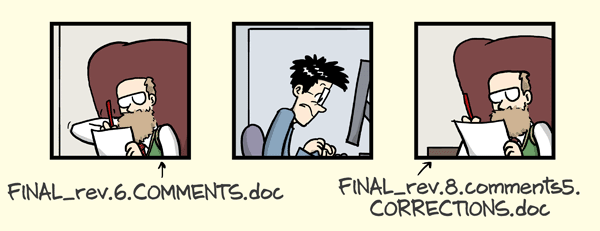
\includegraphics[width=0.9\paperwidth]{figs/phdcomic_finaldoc_2.png}
\end{center}

\url{http://phdcomics.com/comics/archive.php?comicid=1531}
\end{frame}

\begin{frame}[label={sec:org1723665},plain]{}
\begin{center}
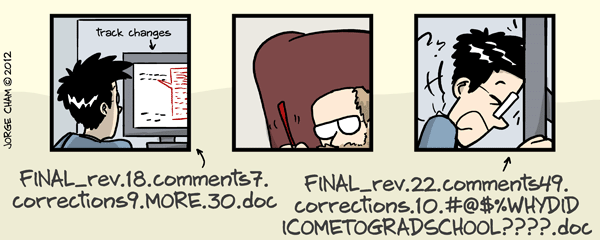
\includegraphics[width=0.9\paperwidth]{figs/phdcomic_finaldoc_3.png}
\end{center}

\url{http://phdcomics.com/comics/archive.php?comicid=1531}
\end{frame}

\begin{frame}[label={sec:org0d505b2}]{¿Qué es el control de versiones y por qué debería importarte?}
\begin{quote}
El control de versiones es un sistema que \alert{registra los cambios}
realizados sobre un archivo o conjunto de archivos a lo largo del
tiempo, de modo que se puedan \alert{recuperar} versiones específicas más
adelante.\footnote{\url{https://git-scm.com/book/es/v1/Empezando-Acerca-del-control-de-versiones}}
\end{quote}
\end{frame}

\begin{frame}[label={sec:org5604d43}]{¿Qué es el control de versiones y por qué debería importarte?}
\begin{quote}
El control de versiones es el cuaderno de laboratorio en el
mundo digital. Es lo que los profesionales usan para realizar un
\alert{seguimiento} de lo que han hecho y para \alert{colaborar} con otras
personas. Cada gran proyecto de desarrollo de software se basa en
ello, y la mayoría de los programadores lo utilizan para sus
trabajos. Y \alert{no sirve sólo para software}: libros, documentos, pequeños
conjuntos de datos y cualquier cosa que cambie con el tiempo o que
deba compartirse puede y debe almacenarse en un sistema de control de
versiones.\footnote{\url{https://swcarpentry.github.io/git-novice/}}
\end{quote}
\end{frame}

\begin{frame}[label={sec:orgf4b3474}]{Viajar en el tiempo}
\begin{itemize}
\item Nada que haya sido sometido a un control de versiones se pierde jamás (\emph{salvo que realmente quieras eliminarlo\ldots{}})
\item \alert{Todas} las versiones antiguas de un fichero se almacenan: un fichero se puede revertir a un estado anterior sin límites.
\end{itemize}
\end{frame}
\begin{frame}[label={sec:org0446962}]{¿Qué? ¿Cuándo? ¿Quién?}
Un sistema de control de versiones registra:
\begin{itemize}
\item El detalle de los cambios realizados.
\item La fecha y hora en la que fueron realizados.
\item La persona que los realizó.
\end{itemize}
\end{frame}

\begin{frame}[label={sec:orgf9578ef}]{Trabajo Colaborativo}
\begin{itemize}
\item Cuando un equipo de personas trabaja conjuntamente en un proyecto, es posible que se produzcan cambios incompatibles en un mismo fichero.
\item El sistema de control de versiones \alert{impide} cambios simultáneos en un fichero. A cambio, permite la \alert{resolución de conflictos} y los documenta.
\end{itemize}
\end{frame}

\subsection{¿Qué son Git y GitHub?}
\label{sec:org9d4ca2d}

\begin{frame}[label={sec:orge3350aa},fragile]{Git es un Sistema de Control de Versiones}
 Git es una herramienta software (accesible mediante línea de comandos con \texttt{git}) que implementa un Sistema de Control de Versiones.

Cada vez que se ejecuta un cambio en una estructura de ficheros controlada con Git, realiza una \guillemotleft{}foto\guillemotright{} del estado de los archivos en ese momento, y guarda una referencia a esa instantánea. Por eficiencia, Git no almacena los archivos sin modificaciones sino un enlace al archivo anterior idéntico que ya está almacenado

\begin{center}
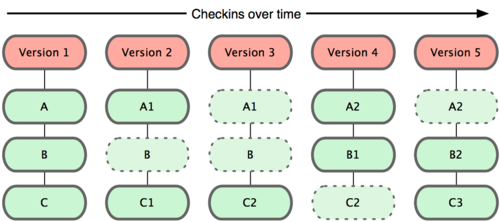
\includegraphics[width=.9\linewidth]{figs/git_model.png}
\end{center}
\end{frame}

\begin{frame}[label={sec:org0bc772f}]{Los estados de Git}
\begin{itemize}
\item El desarrollador incorpora uno o varios ficheros al control de versiones. (\emph{tracked})
\item Realiza modificaciones en los ficheros (\emph{modified}).
\item Incorpora esos ficheros modificados al área de preparación (\emph{staged}).
\item Finalmente, confirma todos los cambios del área de preparación: se realiza la instantánea de los ficheros. (\emph{committed})
\end{itemize}
\begin{center}
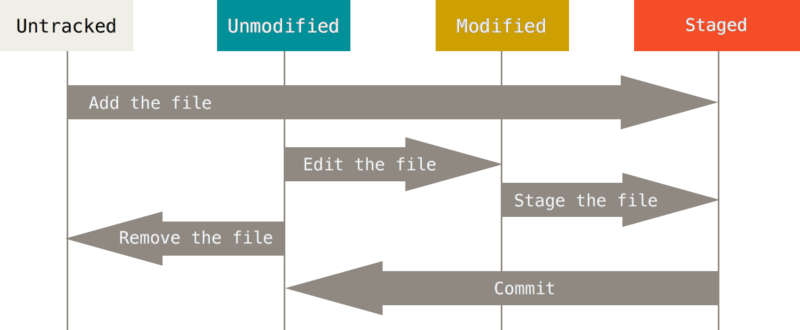
\includegraphics[height=0.4\textheight]{figs/git_estados.png}
\end{center}
\end{frame}

\begin{frame}[label={sec:org4a264d8},fragile]{¿Qué es GitHub?}
 GitHub es la plataforma de alojamiento de código más importante a nivel mundial. Emplea el sistema de control de versiones \texttt{git}, y ofrece una amplia variedad de funcionalidades para el alojamiento y revisión del código, el trabajo colaborativo, y la publicación de páginas web asociadas al repositorio de código.
\end{frame}

\section{Primeros pasos}
\label{sec:orga552806}
\url{https://help.github.com/desktop/guides/}
\subsection{Creación de una cuenta en GitHub}
\label{sec:orgd466b2f}
\subsection{Configuración del ordenador para el uso de la cuenta}
\label{sec:org01023cf}
\subsection{Mi primer repositorio: crear y clonar}
\label{sec:orged19a24}
\section{Flujo de trabajo con \texttt{git} y \texttt{GitHub}}
\label{sec:org712a2b6}
\subsection{Realizar y confirmar cambios (\texttt{add} y \texttt{commit})}
\label{sec:org54e605f}
\subsection{Publicar cambios (\texttt{push})}
\label{sec:orgeb15cc7}
\subsection{Recibir cambios de un repositorio remoto y combinar con una copia local (\texttt{fetch}, \texttt{merge} y \texttt{pull})}
\label{sec:org8dfcc0e}
\section{Trabajo en colaboración}
\label{sec:org7b755aa}
\subsection{Ramas (\texttt{branch})}
\label{sec:orgb8fcd4a}
\subsection{Combinación de código (\texttt{pull request} y \texttt{merge})}
\label{sec:org83e99bb}
\subsection{Tareas y tableros de discusión (\texttt{issues})}
\label{sec:orgb7adb99}
\subsection{Herramientas gráficas para el análisis de un repositorio}
\label{sec:org856f7ae}
\section{GitHub Classroom}
\label{sec:orgca0511c}
\section{Publicación de páginas web en GitHub}
\label{sec:orge43bb83}
\end{document}